\documentclass{beamer}
%[hyperref={colorlinks, citecolor=hltyellow, linkcolor=hltdarkgreen,
  %urlcolor=hltdarkgreen}]
\usepackage[utf8]{inputenc}
\usepackage[backend=bibtex,natbib=true,style=authoryear,backref=true]{biblatex}%autocite=superscript
\renewcommand*{\bibfont}{\footnotesize}
\bibliography{../../paper/Common/Bib/ml}
\usepackage{lmodern}
\usepackage[T1]{fontenc}
\usepackage{booktabs}
\usepackage{mathabx}
%\usepackage{mathtools}
%\usepackage[all]{xy}
\usepackage{graphicx}
\usepackage{tikz}
\usepackage{balance}
\usepackage{tikz-qtree}
\usepackage{longtable}
\usepackage{multirow}
\usepackage{mathtools}

\usepackage{pgfplots}
\pgfplotsset{%compat=1.11,
  /pgfplots/ybar legend/.style={
    /pgfplots/legend image code/.code={%
      %\draw[##1,/tikz/.cd,yshift=-0.25em]
      %(0cm,0cm) rectangle (3pt,0.8em);},
      \draw[##1,/tikz/.cd,bar width=3pt,yshift=-0.2em,bar shift=0pt]
      plot coordinates {(0cm,0.8em)};},
    },
} 
\usetheme{hlt}
%\usecolortheme{rose}
%\definecolor{hltblue}{RGB}{3,61,92}
\definecolor{hltdarkgreen}{RGB}{26,148,129}
%\definecolor{hltlightgreen}{RGB}{155,204,147}
%\definecolor{hltyellow}{RGB}{252,238,166}
%\usecolortheme[named=hltblue]{structure}
%\setbeamercolor{alerted text}{fg=hltdarkgreen}
%\setbeamercolor{example text}{fg=hltlightgreen}

%work-around for citation colour with Beamer + Hyperref + Natbib
\let\oldbibitem=\bibitem
\renewcommand{\bibitem}[2][]{\label{#2}\oldbibitem[#1]{#2}}
\let\oldcite=\cite
%\renewcommand\cite[1]{\hypersetup{linkcolor=hltblue} \hyperlink{#1}{\oldcite{#1}}}
\let\oldcitep=\citep
%\renewcommand\citep[1]{\hypersetup{linkcolor=hltblue}\hyperlink{#1}{\oldcitep{#1}}}
\let\oldciteauthor=\citeauthor
%\renewcommand\citeauthor[1]{\hypersetup{linkcolor=hltblue}\hyperlink{#1}{\oldciteauthor{#1}}}

\newcommand{\bull}[1]{\begin{itemize}\item #1 \end{itemize}}
\newcommand{\fl}{\texttt{4lang}}
\newcommand{\jiweil}{\texttt{mutli}}
\newcommand{\huang}{\texttt{huang}}
\newcommand{\neela}{\texttt{neela}}
\newcommand{\adagram}{\texttt{AdaGram}}
\newcommand{\mutli}{\texttt{mutli}}
\newcommand{\osub}{\texttt{OSub}}

\title{Do multi-sense word embeddings learn more senses?}

\newcommand{\Ro}{\mathbb{R}^{d_1}}
\newcommand{\Rt}{\mathbb{R}^{d_2}}
\newcommand{\any}{\texttt{any}}
\newcommand{\disamb}{\texttt{disamb}}
\newcommand{\e}{$^E$}
\newcommand{\id}{$^I$}
\newcommand{\s}{$^S$}

\newcommand{\logoheight}{1cm}

\author{Márton Makrai}
%[Makrai Márton]{
%  Makrai Márton \\
%\vspace{5mm}
%\includegraphics[height=\logoheight]{../../paper/Common/Logo/nytud.png}
%\hspace{5mm}
%    \includegraphics[height=\logoheight]{../../paper/Common/Logo/hlt/blue_white_bg.png} \\ 
%  }
\date{K + K = 120 Workshop}
%[Fiatal kutatók félidőben 2017]{
%  témavezető: Kornai András\\
%    \vspace{2mm}
%  Fiatal kutatók félidőben \\
%2017. szeptember 28.}
\begin{document}
\AtBeginSection[]{
  \begin{frame}{Áttekintés}
    \tableofcontents[currentsection,subsectionstyle=shaded]
  \end{frame}
}

\maketitle


\begin{frame}{Áttekintés}
  \tableofcontents
\end{frame}

% a) a témát, a releváns hazai és nemzetközi szakirodalmat (20%) 3 dia
% b) kutatásának célját, a kutatási kérdéseket, a hipotéziseket (5%) 1 dia
% c) módszertant, amelyre a kutatás épül (20%) 3 dia
% d) eredményeket (ahol lehet, szemléltesse ábrákkal) (35%) 5 dia
% e) következtetéseket, amelyek az eredmények alapján levonhatók (18%) 2 dia
% f) Az előadást záró diaképen összegezze eddigi publikációit

\section{Szóbeágyazások}

\begin{frame}{Mesterséges ideghálók}
  \centering \includegraphics[width=.7\textwidth]{../../paper/misc/makrai/fiatal/felido/img/deep_neural_network}
  \begin{itemize}
    \item kibernetika (1949), konnekcionizmus (1974), mély tanulás (2006)
    \item feature-ök tanulása, egyre absztraktabb rétegek
    \item 
      \begin{itemize} 
        \item gépi látás \citep{Krizhevsky:2012} 
        \item beszédfelismerés \citep{Hinton:2012}
      \end{itemize}
    \item gyors tanulás a grafikus kártyán
    \item mint az agyban?
  \end{itemize}
\end{frame}
\begin{frame}{Szóbeágyazások (\emph{word embeddings})}
  \begin{itemize}
    \item szavak reprezentációja ideghálókban
    \item vektor: a tér pontjai számsorozatokként
    \item 300 dimenzió
    \item szóalak $\mapsto$ vektor
    \item hasonló eloszlású szó $\mapsto$ közeli pont
      \bull{eloszlás: milyen kontextusokban milyen gyakori}
      %\item változatok
      %\begin{itemize}
    \item milliárd szavas korpuszokon tanítjuk (\emph{giga-word corpus}),  \\
      pl.~\cite{Halacsy:2004,Oravecz:2014}
    \item word2vec, skip-gram, continuous bag of words \citep{Mikolov:2013d}
      %\item GloVe \citep{Pennington:2014}
      %\end{itemize} 
    \item közös reprezentáció \citep{Collobert:2011,Hashimoto:2017}
    \item kompozíció: karakter, morféma, szó, query, mondat, retorika
      \begin{itemize}
        \item morfémák \citep{Lazaridou:2013}
        \item szó alatti: fastText \citep{Bojanowski:2016}
        \item gondolatvektor \citep{Vaswani:2017}
      \end{itemize}
  \end{itemize}
\end{frame}
\begin{frame}{Jelentésfelbontás vektorokkal}{\citep{Mikolov:2013l}}
         \cite{Katz:1963}
  \includegraphics[width=\textwidth]{../../paper/misc/makrai/fiatal/felido/img/analogy}
      \[\text{\bf király} + \text{\bf nő} - \text{\bf férfi} \approx 
      \text{\bf királynő}\]
      \begin{itemize}
        \item legközelebbi szomszéd (NN)
        %\item más relációk?
      \end{itemize}
\end{frame}


\begin{frame}%{Lineáris fordítás}
  {Szavak fordítása \citep{Mikolov:2013x}}
    \begin{columns}
      \begin{column}{.4\textwidth}
        \begin{figure}
          \centering
          \includegraphics[width=\columnwidth]{../../paper/misc/makrai/mtu15/img/red-pill} 
        \end{figure}
      \end{column}
      \pause
      \begin{column}{.6\textwidth}
        \begin{itemize}
          \item két vektortér között a legegyszerűbb leképezés a lineáris (mátrix)
          \item most két nyelv beágyazása között
            %\[W: \Ro \rightarrow \Rt \quad z \approx Wx\]
          \item a fordítási leképezés tanítása néhány~ezer szópáron + teszt
            \[\min_W \sum_i || Wx_i - z_i ||^2 \]
        \end{itemize}
      \end{column}
    \end{columns}
    \begin{figure}
      \includegraphics[width=.9\textwidth]{../../paper/misc/makrai/fiatal/skip_gram_mapping}
    \end{figure}
\end{frame}

\section{Több jelentés}

\begin{frame}{Szótöbbértelműség}
  \begin{itemize}
    \item homonímia: \emph{ár} `ellenérték; zúdulás`
    \item poliszémia
      \begin{itemize}
        \item metonímia: \emph{iskola} (emberek, épület)
        \item rendszertelen: \emph{nap} (időszak, égitest)
      \end{itemize}
    \item a különbség alapja
      \begin{itemize} 
        \item etimológia, ha van
        \item kapcsolat a jelentések között (nem empirikus)
      \end{itemize}

    \item poliszémiagráfok, hasonlóság nyelvek között \citep{Youn:2016}
      \begin{itemize}
        \item mely fogalmak poliszémek gyakran
        \item fogalomklaszterek
      \end{itemize}
    \item szófaji különbség (\emph{vár})
  \end{itemize}
\end{frame}
\begin{frame}{Szójelentés-klaszterezés}
  \begin{tabular}{lll}
    word sense disambiguation (WSD) & osztályozás & felügyelt \\
      word sense induction (WSI) \citep{Schutze:1998} & klaszterezés & felügyeletlen \\
  \end{tabular}
    \begin{itemize}
      \item többjelentésű vektoros szómodell \citep{Reisinger:2010}
      \item ideghálóval \citep{Huang:2012}
      \item szabadon elérhető, hatékony eszköz \citep{Neelakantan:2014}
      \item Dirichlet-folyamatként 
        \begin{itemize}
          \item \cite{Li:2015}
          \item jelentések összevonása tanuláskor \citep{Bartunov:2015}
        \end{itemize}
      \item elvileg érdekes, de túl finom a felbontás (duplumok)
      \item a paraméterek számát kontrollálva kis javulás szemantikai
        feladatokban \citep{Li:2015}
    \end{itemize}
\end{frame}

%\section{A jelentések számának eloszlása}

%\begin{frame}[fragile]{A jelentések számának eloszlása}
%  Közös munka Borbély Gáborral, Nemeskey Dáviddal és Kornai Andrással
%  \newcommand{\lexdistri}[7]{
%    \addplot[style={fill=#7}]
%    %bblue, mark=none
%    coordinates {(CED,#1) (LDOCE,#2) (OEn,#3) (EKSZ,#4) (NSZ,#5) (OHu,#6) };
%  }
%  \begin{table}
%    {\tiny
%    \begin{tikzpicture}
%      \begin{axis}[
%          ymode = log,
%        log origin=infty,
%        width  = 0.9*\textwidth,
%        height = .5\textheight,
%        %8cm, %major x tick style = transparent,
%        ybar=0pt,%=2*\pgflinewidth,
%        bar width=5pt,
%        %ymajorgrids = true, %ylabel = {Run time speed}, %symbolic x coords={EgyptHD,Hover,Navi},
%        symbolic x coords={CED,LDOCE,OEn,EKSZ,NSZ,OHu},
%        xtick = data,
%        %scaled y ticks = false, %enlarge x limits=0.25, %ymin=0, %legend cell align=left, %
%        legend style={ at={(1.05,1.05)}, anchor=north west, column sep=1ex }
%      ]
%        \lexdistri{0.98}{0.88}{0.77}{0.55}{0.93}{0.94}{hltblue}
%        \lexdistri{0.02}{0.11}{0.20}{0.01}{0.02}{0.05}{hltdarkgreen}
%        \lexdistri{0.00}{0.01}{0.03}{0.00}{0.00}{0.00}{hltlightgreen}
%        \lexdistri{0.00}{0.00}{0.01}{0.00}{0.00}{0.00}{hltyellow}
%        \lexdistri{0.00}{0.00}{0.00}{0.00}{0.00}{0.00}{black}
%        \lexdistri{0.00}{0.00}{0.00}{0.00}{0.00}{0.00}{grey}
%        \legend{1,2,3,4,5,6+}
%      \end{axis}
%    \end{tikzpicture}
%    }
%
%    \newcommand{\embeddistri}[7]{
%      \addplot[style={fill=#7}]
%      %bblue,mark=none
%    coordinates {(AdaGramEn,#1) (huang,#2) (neelaNP6k,#3) (AdaGram,#4)
%    (jiweil,#5) (neelas2,#6)
%    };
%  }
%    {\tiny
%      \begin{tikzpicture}
%        \begin{axis}[
%            ymode = log,
%          log origin=infty,
%          width  = .9\textwidth,
%          height = .5\textheight,
%          %major x tick style = transparent,
%          ybar=0pt,%=2*\pgflinewidth,
%          bar width=5pt,
%          %ymajorgrids = true,
%          %ylabel = {Run time speed},
%          %symbolic x coords={EgyptHD,Hover,Navi},
%          symbolic x coords={AdaGramEn,huang,neelaNP6k,AdaGram,jiweil,neelas2},
%          %xtick = data,
%          %scaled y ticks = false,
%          %enlarge x limits=0.25,
%          %ymin=0,
%          %legend cell align=left,
%          legend style={ at={(1.05,1.05)}, anchor=north west, column sep=1ex }
%        ]
%          \embeddistri{0.26}{0.94}{0.95}{0.57}{0.20}{7.74}{hltblue}
%          \embeddistri{0.69}{0.00}{0.03}{0.32}{0.32}{0.04}{hltdarkgreen}
%          \embeddistri{0.02}{0.00}{0.01}{0.06}{0.26}{0.00}{hltlightgreen}
%          \embeddistri{0.01}{0.00}{0.00}{0.02}{0.14}{0.00}{hltyellow}
%          \embeddistri{0.02}{0.00}{0.00}{0.03}{0.05}{0.00}{gray}
%          \embeddistri{0.00}{0.06}{0.00}{0.00}{0.02}{0.00}{white}
%          \legend{1,2,3,4,5,6+}
%        \end{axis}
%      \end{tikzpicture}
%      }
%\end{table}
%\end{frame}
%\begin{frame}{Problémák}
%  \begin{itemize}
%    \item ferde eloszlás
%      \begin{itemize}
%        \item majdnem minden szó egyjelentésű
%        \item osztályozás: $\pm$többértelmű, F-pontszám
%      \end{itemize}
%    \item gyakorisági hatás
%      \bull{Zipf-törvény többértelműségre \citep{Manin:2008}}
%  \end{itemize}
%\end{frame}
%\begin{frame}
%  \begin{table}[!b]
%    \resizebox{.45\framewidth}{!}{%
%      \begin{tabular}{l|rc}
%        \toprule
%            Resources compared & $n$ & $\rho$\\
%            \midrule
%            LDOCE vs CED & 23702 & 0.266 \\
%            EKSZ vs NSZ (b) & 3484 & 0.648 \\
%            \midrule
%            \neela.30k vs CED & 23508 & 0.089 \\
%            \neela.NP.6k vs CED & 23508 & 0.084 \\
%            \neela.NP.30k vs CED & 23508 & 0.112 \\
%            \neela.30k vs LDOCE &  21715 & 0.226 \\
%            \neela.NP.6k vs LDOCE  & 21715 & {\bf 0.292} \\
%            \neela.NP.30k vs LDOCE & 21715 & 0.278 \\
%            \huang\ vs CED & 23706 & 0.078 \\
%            \huang\ vs LDOCE & 21763 & {\bf 0.280} \\
%            \neela.s4 vs EKSZ & 45401 & 0.067 \\
%            \jiweil\ vs EKSZ & 32007 & 0.023 \\
%            AdaGram vs EKSZ & 26739 & 0.086 \\
%            AdaGram.a05 vs EKSZ & 26739 & 0.088 \\
%            %\midrule
%            %\neela.30k vs \huang  & 99156 & 0.349 \\
%            %\neela.NP.6k vs \huang & 99156 & {\bf 0.901} \\
%            %\neela.NP.30k vs \huang & 99156 & 0.413 \\
%            %\neela.s4 vs \jiweil & 283083 & 0.123 \\
%            %AdaGram vs \neela.s4 & 199370 & {\bf 0.389} \\
%            %AdaGram vs \jiweil & 201291 & 0.140 \\
%            \bottomrule
%      \end{tabular}
%        }
%        %\caption{Word sense distribution similarity between various resources}
%        \label{tab:corrHu}  \label{tab:corrEn}
%        \resizebox{.45\framewidth}{!}{%
%          \begin{tabular}{l|rc}
%            \toprule
%            Resources compared & $n$ & $\rho$\\
%            \midrule
%            %CED vs POS & 42532 & 0.052 \\
%            %LDOCE vs POS & 28549 & {\bf 0.206} \\
%            %\osub vs POS  & 48587 & {\bf 0.141} \\
%            %EKSZ vs POS  & 52158 & 0.080 \\
%            %NSZ vs POS  & 3532 & 0.046 \\
%            %\huang\ vs POS & 98405 & 0.026\\
%            %\midrule
%            AdaGram vs freq & 399985 & 0.343 \\
%            \huang\ vs freq & 94770 & 0.376 \\
%            CED vs freq  & 36709 & 0.124 \\
%            LDOCE vs freq  & 27859 & 0.317 \\
%            \neela.s4 vs freq &  94044 & {\bf 0.649} \\
%            \neela.NP.30k vs freq  & 94044 & 0.368 \\
%            \neela.NP.6k vs freq  & 94044 & {\bf 0.635}\\
%            UMBC POS vs freq & 136040 & -0.054\\
%            \bottomrule
%          \end{tabular}
%        }
%  \end{table}
%      \begin{itemize}
%        \item freq $\approx$ MSE $\napprox$ CED
%      \end{itemize}
%\end{frame}
%\begin{frame}{A gyakoriság hatását kivonva (részleges korreláció)}
%  \begin{table}
%    \resizebox{.9\textwidth}{!} {
%      \begin{tabular}{l|rcrcrc}
%        \toprule
%        &\multicolumn{2}{c}{\textbf{CED}} &\multicolumn{2}{c}{LDOCE} &\multicolumn{2}{c}{\osub}\\
%        \midrule
%        CED	& 36709	& 1.0	& 22375	& \textbf{0.546}	& 20937	& -0.365	\\
%        LDOCE	& 22375	& \textbf{0.546}	& 27859	& 1.0	& 19283	& -0.002	\\
%        \osub	& 20937	& -0.365	& 19283	& -0.002	& 58296	& 1.0	\\
%        \midrule
%        AdaGram umbc	& 36709	& -0.344	& 27859	& -0.307	& 58296	& 0.267	\\
%        cmultivec umbc	& 25231	& \textbf{0.844}	& 23702	& 0.521	& 39965	& -0.485	\\
%        %cmultivec umbc.z05.s95	& 25231	& 0.620	& 23702	& 0.363	& 39965	& -0.392	\\
%        \huang release	& 23600	& 0.274	& 21734	& 0.312	& 42331	& -0.207	\\
%        %huang release.z05.s95	& 23600	& 0.270	& 21734	& 0.310	& 42331	& -0.207	\\
%        %\neela MSSG.300D.30K	& 23423	& -0.237	& 21688	& -0.137	& 42325	& 0.125	\\
%        \neela NP-MSSG.300D.6K	& 23423	& 0.331	& 21688	& 0.350	& 42325	& -0.252	\\
%        \neela NP-MSSG.50D.30K	& 23423	& -0.307	& 21688	& -0.119	& 42325	& 0.168	\\
%        \neela umbc	& 36709	& 0.536	& 27859	& 0.411	& 58296	& -0.349\\
%        \toprule
%        &\multicolumn{2}{c}{EKSZ} &\multicolumn{2}{c}{NSZ (b)} &\multicolumn{2}{c}{\osub}\\
%        \midrule
%        EKSZ	& 33235	& 1 0	& 1680	& \textbf{0.950}	& 17336	& -0.313	\\
%        NSZ b	& 1680	& \textbf{0.950}	& 1999	& 1.0	& 995	& -0.318	\\
%        \osub	& 17336	& -0 313	& 995	& -0.318	& 76876	& 1.0	\\
%        \midrule
%        AdaGram a05 Webkorpusz	& 26739	& 0.411	& 1535	& 0.506	& 67212	& -0.012	\\
%        AdaGram Webkorpusz	& 26739	& -0.576	& 1535	& -0.451	& 67212	& 0.186	\\
%        %jiweil webkorp.sense.context	& 31411	& -0.044	& 1863	& -0.020	& 74450	& 0.022	\\
%        %jiweil webkorp.sense.context.z05.s95	& 31411	& -0.044	& 1863	& -0.021	& 74450	& 0.022	\\
%        \jiweil Webkorpusz & 31411	& -0.044	& 1863	& -0.020	& 74450	& 0.022	\\
%        %jiweil webkorp.sense.z05.s95	& 31411	& -0.263	& 1863	& -0.299	& 74450	& 0.025	\\
%        \neela Webkorpusz	& 33182	& \textbf{0.658}	& 1995	& \textbf{0.744}	& 76758	& -0.085	\\
%        \bottomrule
%      \end{tabular}
%    }
%  \end{table}
%\end{frame}

\begin{frame}{Lineáris fordítás többjelentésű embeddingből}
  \begin{itemize}
    \item elv: más jelentés, más fordítás
      \bull{de szinonim fordítások}
    \item a célembedding marad egyjelentésű
      \citep{Pennington:2014,Mikolov:2013f}
    \item tanítás az első jelentésen 
      \bull{szótár: \citep{Acs:2013}}
  \end{itemize}
  \begin{figure}
    \centering
      \resizebox{\textwidth}{!} {
        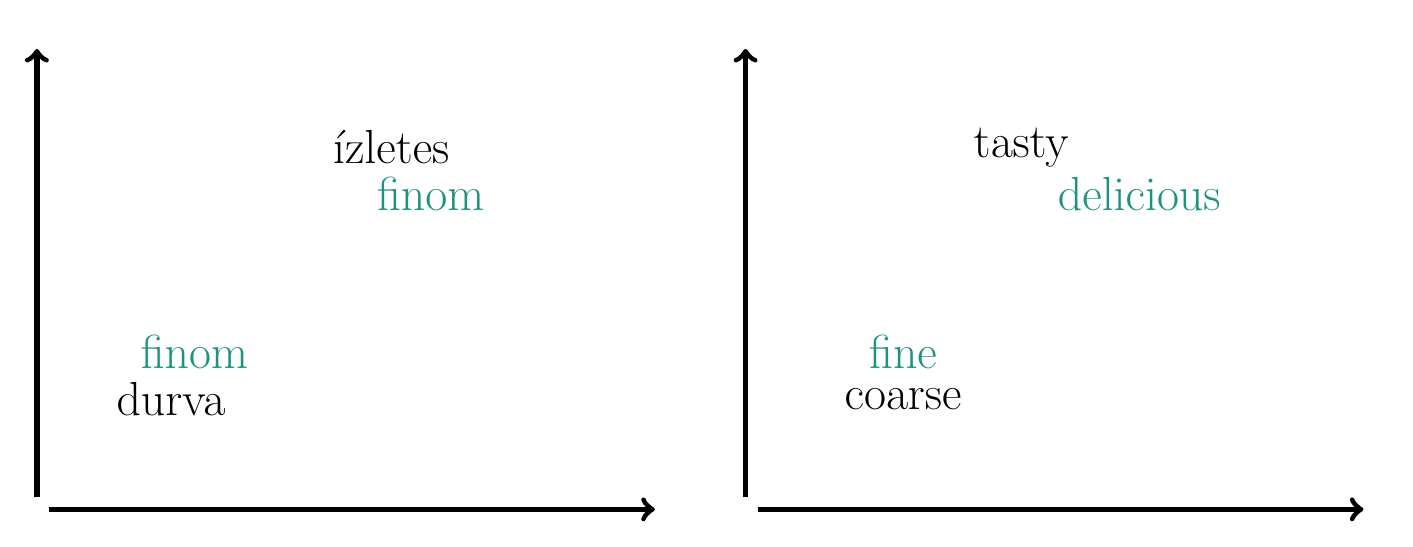
\begin{tikzpicture}[line width=2pt] %[&gt;=stealth']
          \tikzstyle{every node}=[font=\LARGE]
          %\tikzset{every edge thick}
            \node[text=hltdarkgreen] (hf) at (2, 2) {finom};
            \node (hf) at (1.7, 1.4)  {durva};
            \node[text=hltdarkgreen] (hs) at (5, 4)  {finom};
            \node (hs) at (4.5, 4.6)  {ízletes};
            \node[text=hltdarkgreen] (gf) at (11, 2) {fine};
            \node (gf) at (11, 1.4) {coarse};
            \node[text=hltdarkgreen] (gs) at (14, 4) {delicious};
            \node (gs) at (12.5, 4.6) {tasty};
            \node (ho) at (0, 0) {};
            \node (hx) at (8, 0) {};
            \node (hy) at (0, 6) {};
            \node (go) at (9,0) {};
            \node (gx) at (17,0) {};
            \node (gy) at (9,6) {};

            \draw[->] (ho) edge (hx);
            \draw[->] (ho) edge (hy);
            \draw[->] (go) edge (gx);
            \draw[->] (go) edge (gy);
        \end{tikzpicture}
      }
      % \caption{Linear translation of word senses. The Hungarian word
      % \emph{finom} is ambiguous between `fine' and `delicious'.}
      % \label{fig:AdaGram}
  \end{figure}
\end{frame}
\begin{frame}[allowframebreaks]{Kiértékelés}
  \begin{itemize}
        \item  különböző vektor $\xRightarrow ?$ különböző jelentés
        \item a paraméterek és a célembedding választása
          \bull{jónak vesszük, ha legalább egy jelentésvektornak van jó
          fordítása}
        \item két vektor jó fordításainak halmaza legyen különböző
        \item ilyenek arányát nézzük az többértelműnek jósoltak között
  \end{itemize}
\end{frame}
\begin{frame}
  \begin{table}
    %\resizebox{\columnwidth}{!}{%
    \begin{tabular}{lcccc|cc}
      \toprule
        & dim & $\alpha/\gamma$ & $p$ & $m$ & any & disamb \\
        % & \multicolumn{6}{c|}{forward NN search} & \multicolumn{6}{c}{reverse NN search} \\
        %vocab cutoff &&&&& \multicolumn{2}{c}{8192} & \multicolumn{2}{c}{16384} & \multicolumn{2}{c|}{32768} & \multicolumn{2}{c}{8192} & \multicolumn{2}{c}{16384} & \multicolumn{2}{c}{32768} \\
        \midrule
        %/jiweil/mnsz/stemmed/mnsz-stemmed-CRP-800-w15-joint_vect_sense.mse 23.0% 2.200%
        %/jiweil/mnsz/stemmed/mnsz-stemmed-CRP-800-w15-joint_vect_sense_context.mse 26.1% 3.300%
        %/neelakantan/mnsz/stemmed/mnsz2-stemmed-neela-np-800-s2_cluscent.mse 36.3% 6.400%
        %/neelakantan/webkorp_1-sense_sense.mse 37.8% 5.900%
        %/neelakantan/mnsz/stemmed/mnsz2-stemmed-neela-np-800-s2_sense.mse 38.1% 6.500%
        HNC	        & 800	& .02	&       & 100   & 48.5\%	&  7.6\% \\
        \neela~Wk&300&--&2   &big  & 54.0\%	&  12.4\% \\
        HNC stem & 800	& .05	&       &  big & 55.1\%	&  10.4\% \\
        %	& \mutli~Webkorp\footnotemark  &&&&    & 1.0 & 55.0% 13.5\% \\
        HNC         & 160 & .05 & 3     & 200   & 62.2\%	&  15.0\% \\
        \mutli~Wk &300&.25 &       & 71    & 62.9\%	&  17.4\% \\
        Webkorpusz	    & 800	& .05	&       & 100	  & 65.9\%	&  17.4\% \\
        HNC	        & 600	& .05	& 5     & 100	  & 68.6\%	&  16.6\% \\
        HNC	        & 600	& .1  & 3     & 50	  & 69.1\%	&  18.8\% \\
        Webkorpusz	    & 800	& .1  &       & 100	  & 73.9\%	&  23.9\% \\
        \bottomrule
    \end{tabular}
    %}
  \end{table}
\end{frame}

  \begin{frame}[allowframebreaks]{Jó fordítások hasonlósága} 
    \small
    \begin{longtable}{lllll}
      %\setlength{\tabcolsep}{3pt}
      %\resizebox{\textwidth}{!}{%
      %\centering
      \toprule
      %&$s$     &         &                       & covg \\
      %\midrule
        E	& -0.04849	& függő	& addict, aerial	& 0.4 \\
        S	& 0.01821	& alkotó	& constituent, creator	& 0.5 \\
        S	& 0.05096	& előzetes	& preliminary, trailer	& 1.0 \\
        S	& 0.0974	& kapcsolat	& affair, conjunction, linkage	& 0.33 \\
        I	& 0.1361	& kocsi	& coach, carriage	& 1.0 \\
        S	& 0.136	& futó	& runner, bishop	& 1.0 \\
        S	& 0.1518	& keresés	& quest, scan	& 0.67 \\
        S	& 0.1574	& látvány	& outlook, scenery, prospect	& 0.6 \\
        S	& 0.1626	& fogad	& bet, greet	& 1.0 \\
        S	& 0.1873	& induló	& march, candidate	& 1.0 \\
        I	& 0.187	& nemes	& noble, peer	& 0.67 \\
        E	& 0.1934	& eltérés	& variance, departure	& 0.4 \\
        E	& 0.1943	& alkalmazás	& employ, adaptation	& 0.33 \\
        S	& 0.2016	& szünet	& interval, cease, recess	& 0.43 \\
        E	& 0.2032	& kezdeményezés	& initiation, initiative	& 1.0 \\
        S	& 0.2052	& zavar	& disturbance, annoy, disturb, turmoil	& 0.57 \\
        S	& 0.2054	& megelőző	& preceding, preventive	& 0.29 \\
        IE& 0.2169	& csomó	& knot\id, lump\id, mat\e	& 1.0  \\
        E\footnotemark
        & 0.21	& remény	& outlook, promise, expectancy	& 0.6	  \\
        S	& 0.2206	& bemutató	& exhibition, presenter	& 0.67 \\
        E	& 0.2208	& egyeztetés	& reconciliation, correlation	& 0.5 \\
        S	& 0.237	& előadó	& auditorium, lecturer	& 0.67 \\
        E	& 0.2447	& nyilatkozat	& profession, declaration	& 0.4 \\
        I	& 0.2494	& gazda	& farmer, boss	& 0.67 \\
        I	& 0.2506	& kapu	& gate, portal	& 1.0 \\
        I	& 0.2515	& előbbi	& anterior, preceding	& 0.67 \\
        I	& 0.2558	& kötelezettség	& engagement, obligation	& 0.67 \\
        E	& 0.265	& hangulat	& morale, humour	& 0.5 \\
        E	& 0.2733	& követ	& succeed, haunt	& 0.67 \\
        SE	& 0.276	& minta	& norm\s, formula\e, specimen\s	& 0.75  \\
        S	& 0.2807	& sorozat	& suite, serial, succession	& 1.0 \\
        S	& 0.2935	& durva	& coarse, gross	& 0.18 \\
        I	& 0.3038	& köt	& bind, tie	& 0.67 \\
        E	& 0.3045	& egyezmény	& treaty, protocol	& 0.67 \\
        I	& 0.3097	& megkülönböztetés	& discrimination, differentiation	& 0.5 \\
        I	& 0.309	& ered	& stem, originate	& 0.5 \\
        I	& 0.319	& hirdet	& advertise, proclaim	& 1.0 \\
        E	& 0.3212	& tartós	& substantial, durable	& 1.0 \\
        I	& 0.3218	& ajánlattevő	& bidder, supplier, contractor	& 0.6 \\
        I	& 0.3299	& aláírás	& signing, signature	& 0.67 \\
        I	& 0.333	& bír	& bear, possess	& 1.0 \\
        I	& 0.3432	& áldozat	& sacrifice, victim, casualty	& 1.0 \\
        IE	& 0.3486	& kerület	& ward\id, borough\id, perimeter\e	& 0.3  \\
        I	& 0.3486	& utas	& fare, passenger	& 1.0 \\
        I	& 0.3564	& szigorú	& stern, strict	& 0.5 \\
        I	& 0.3589	& bűnös	& sinful, guilty	& 0.5 \\
        I	& 0.3708	& rendes	& orderly, ordinary	& 0.5 \\
        I	& 0.3824	& eladó	& salesman, vendor	& 0.5 \\
        I	& 0.3861	& enyhe	& tender, mild, slight	& 0.6 \\
        I	& 0.3897	& maradék	& residue, remainder	& 0.33 \\
        I	& 0.3986	& darab	& chunk, fragment	& 0.4 \\
        E	& 0.4012	& hiány	& poverty, shortage	& 0.5 \\
        %I	& 0.4093	& kutatás	& exploration, quest	& 0.5 \\
        %I	& 0.4138	& tanítás	& tuition, lesson	& 0.67 \\
        %I	& 0.4196	& őszinte	& frank, sincere	& 0.67 \\
        %I	& 0.4229	& környék	& neighborhood, surroundings, vicinity	& 0.38 \\
        %I	& 0.4446	& ítélet	& judgement, sentence	& 0.67 \\
        %I	& 0.4501	& gyerek	& childish, kid	& 0.67 \\
        %I	& 0.4521	& csatorna	& ditch, sewer	& 0.4 \\
        %I	& 0.4547	& felügyelet	& surveillance, inspection, supervision	& 0.43 \\
        %E	& 0.4551	& ritka	& rare, odd	& 0.5 \\
        %S	& 0.4563	& szerető	& fond, lover, affectionate, mistress	& 0.67 \\
        %I	& 0.4608	& szeretet	& affection, liking	& 0.67 \\
        %I	& 0.4723	& vizsgálat	& inquiry, examination	& 0.67 \\
        %I	& 0.4853	& tömeg	& mob, crowd	& 0.5 \\
        %I	& 0.4903	& puszta	& pure, plain	& 0.22 \\
        %I	& 0.4904	& srác	& kid, lad	& 1.0 \\
        %I	& 0.4911	& büntetés	& penalty, sentence	& 0.29 \\
        %I	& 0.4971	& képviselő	& delegate, representative	& 0.67 \\
        %I	& 0.4975	& határ	& boundary, border	& 0.67 \\
        %I	& 0.5001	& drága	& precious, dear, expensive	& 1.0 \\
        %S	& 0.5093	& uralkodó	& prince, ruler, sovereign	& 0.5 \\
        %I	& 0.5097	& válás	& separation, divorce	& 0.67 \\
        %I	& 0.5103	& ügyvéd	& lawyer, advocate	& 0.67 \\
        %I	& 0.5167	& előnyös	& advantageous, profitable, favourable	& 1.0 \\
        %I	& 0.5169	& merev	& rigid, strict	& 1.0 \\
        %I	& 0.5204	& nyíltan	& openly, outright	& 1.0 \\
        %I	& 0.5217	& noha	& notwithstanding, albeit	& 1.0 \\
        %I	& 0.5311	& hulladék	& litter, garbage, rubbish	& 0.43 \\
        %I	& 0.5311	& szemét	& litter, garbage, rubbish	& 0.43 \\
        %I	& 0.5612	& kielégítő	& satisfying, satisfactory	& 1.0 \\
        %E	& 0.5617	& vicc	& joke, humour	& 1.0 \\
        %I	& 0.5737	& szállító	& supplier, vendor	& 1.0 \\
        %I	& 0.5747	& óvoda	& nursery, daycare, kindergarten	& 1.0 \\
        %I	& 0.5754	& hétköznapi	& mundane, everyday, ordinary	& 0.75 \\
        %I	& 0.5797	& anya	& mum, mummy	& 1.0 \\
        %I	& 0.5824	& szomszédos	& neighbouring, neighbour	& 0.4 \\
        %E	& 0.5931	& szabadság	& liberty, independence	& 1.0 \\
        %I	& 0.6086	& lelkész	& pastor, priest	& 0.4 \\
        %I	& 0.6304	& fogalom	& notion, conception	& 1.0 \\
        %I	& 0.6474	& fizetés	& salary, wage	& 0.67 \\
        %I	& 0.6551	& táj	& landscape, scenery	& 1.0 \\
        %I	& 0.6583	& okos	& clever, smart	& 0.67 \\
        %I	& 0.6707	& autópálya	& highway, motorway	& 0.5 \\
        %I	& 0.6722	& tilos	& prohibited, forbidden	& 1.0 \\
        %I	& 0.6811	& bevezető	& introduction, introductory	& 1.0 \\
        %I	& 0.7025	& szövetség	& coalition, alliance, union	& 0.75 \\
        %I	& 0.7065	& fáradt	& exhausted, tired, weary	& 1.0 \\
        %I	& 0.7066	& kiállítás	& exhibit, exhibition	& 0.67 \\
        %I	& 0.7135	& hirdetés	& advert, advertisement	& 1.0 \\
        %I	& 0.7147	& ésszerű	& rational, logical	& 1.0 \\
        %I	& 0.7664	& logikai	& logic, logical	& 1.0 \\
        %I	& 0.7757	& szervez	& organise, organize, arrange	& 1.0 \\
        %I	& 0.8122	& furcsa	& strange, odd	& 0.4 \\
        %I	& 0.8277	& azután	& afterwards, afterward	& 0.67 \\
        %I	& 0.8689	& megbízható	& dependable, reliable	& 0.67 \\
    \bottomrule
    %}
    % \caption{Hungarian words with the rNN@1 translations of their sense
    % vectors.  The first column is a post-hoc annotation by András Kornai
    % (\emph E error in translation, \emph I identical, \emph S separate
    % meanings), $s$ is the cosine similarity of the translations, and
    % \emph{covg} denotes the coverage of the @1 translations over all gold
    % translations.}
  \end{longtable}
  %\label{tab:alkoto} 
  %{\footnotesize $^7$ The basic translations \emph{hope} is missing}
\end{frame} 
\begin{frame}{Konklúzió}
  \begin{itemize}
    \item input: korpusz két nyelvből és 5 ezer fordítási szópár
    \item előálló erőforrás: egyértelműsített fordítás a korpusz szókincsére
    \item kutatási eredmény: a poliszémia fajtáinak elkülönítése
      koszinuszhasonlósággal (olyan szavakra ellenőriztük, amik ugyanannak a
      szónak a fordításai)
    \item továbblépés: a különféle többjelentésű skip-gram modellek
      szisztematikusabb vizsgálata
  \end{itemize}
\end{frame} 
%\begin{frame}{Az előadó főbb publikációi}
%  \newcommand{\vspacelast}{\vspace{6mm}}
%  \vspacelast
%  \centering\url{https://hlt.bme.hu/makrai}
%  \vspacelast
%  \begin{itemize}
%    \item A \fl~fogalmi szótár \\ \citep{Kornai:2013,Kornai:2015a}
%      \begin{itemize}
%        \item igei szerepek \citep{Makrai:2014}
%        \item a definiáló szókincs \citep{Makrai:2013a,Kornai:2015a}
%        \item aktivációterjedés \citep{Nemeskey:2013}
%      \end{itemize}
%    \item szóbeágyazások
%      \begin{itemize}
%        \item \alert{lexikai relációk} \citep{Makrai:2013b,Makrai:2014b}
%        \item európai nyelvekre \citep{Makrai:2015,Makrai:2015b} % MSZNY, CogInfoCom
%        \item vektorok az agyban \citep{Makrai:2014p}
%        \item többértelműség  háromszögelésben \citep{Makrai:2016l}
%        \item többjelentésű embeddingek (MSEk) \\ (\cite{Borbely:2016}, Makrai (bírálat alatt))
%      \end{itemize}
%  \end{itemize}
%\end{frame}
\begin{frame}[allowframebreaks]{Irodalomjegyzék}
  \printbibliography
\end{frame}
%\begin{frame}%{csoportjaim és témáink}
%  \newcommand{\vspaceaffil}{\vspace{.7cm}}
%  \begin{columns} 
%    \begin{column}{0.1\textwidth}
%      \includegraphics[height=1.3cm]{../../paper/Common/Logo/hlt/blue_white_bg.png}
%    \end{column}
%    \begin{column}{0.8\textwidth}
%      \begin{itemize} 
%        \item témavezető: Kornai András
%        \item csoport: \\ szövegértés mesterséges ideghálókkal és a
%          \fl~szemantikus hálóval
%      \end{itemize}
%    \end{column}
%  \end{columns}
%  \vspaceaffil
%  \begin{columns}
%    \begin{column}{0.1\textwidth}
%      \includegraphics[height=1.3cm]{../../paper/Common/Logo/nytud.png}
%    \end{column}
%    \begin{column}{0.8\textwidth}
%      \begin{itemize}
%        \item MTA NYI, Váradi Tamás
%        \item csoport: \\ a Magyar Nemzeti Szövegtár (milliárd szó), \\ igei szerkezetek,
%          történeti korpuszok, \\ veszélyeztetett nyelvek
%      \end{itemize}
%    \end{column}
%  \end{columns}
%  \vspaceaffil
%  \begin{columns}
%    \begin{column}{0.1\textwidth}
%      \includegraphics[height=1.3cm]{../../logo/mta-ttk-logo-01}
%    \end{column}
%    \begin{column}{0.8\textwidth}
%      \begin{itemize}
%        \item MTA TTK KPI, Balázs László, Ehmann Bea
%        \item izolált csoportban dolgozók naplóinak pszichológiai
%          tartalomelemzése szóbeágyazásokkl
%      \end{itemize}
%    \end{column}
%  \end{columns}
%\end{frame}
\begin{frame}{Mondatszemantika}
  \centering \includegraphics[width=\textwidth]{../../paper/misc/makrai/fiatal/felido/img/montague}
      \bull{igazságfeltételek, modellelmélet \\
      \citep{Montague:1970,Montague:1970a}}
\end{frame}
\begin{frame}{Lexikai felbontás \citep{Katz:1963}}

  \resizebox{\textwidth}{!}{%
    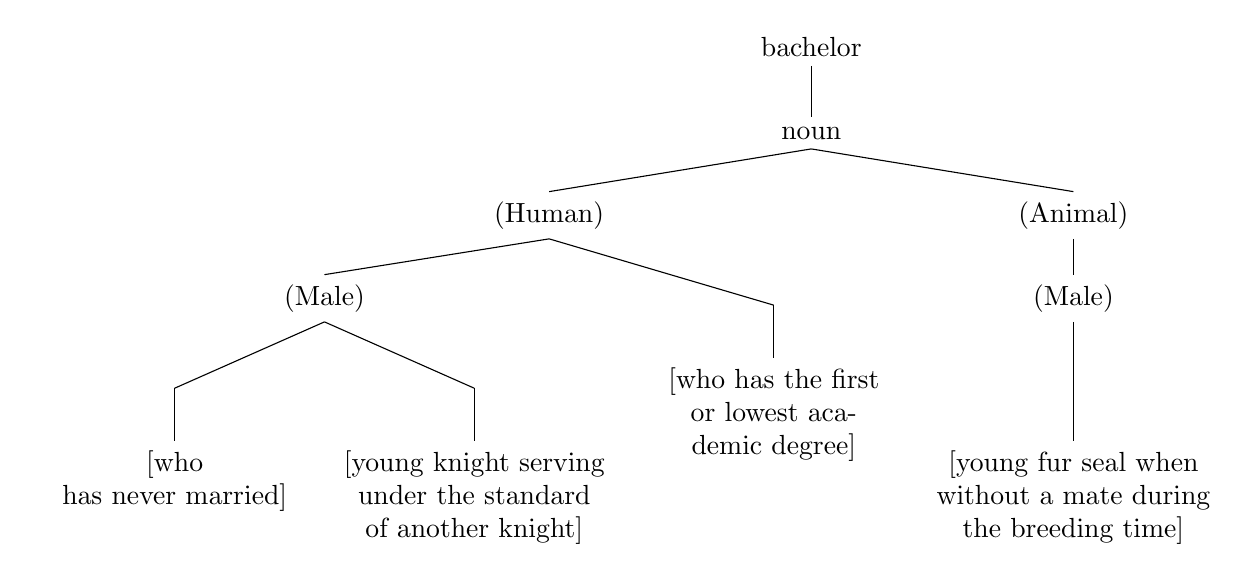
\begin{tikzpicture}%[grow'=right]
      \tikzset{every leaf node/.style={text width=3.5cm}, text centered}
          \Tree
      [.{bachelor}
      [.noun
        [.(Human)
            [.(Male)
                [{[who \\ has never married]} ]
                [{[young knight serving under the standard of another knight]} ]
            ]
            [{[who has the first or lowest academic degree]} ]
        ]
        [.{(Animal)}
            [.{(Male)}
                [{[young fur seal when without a mate during the breeding time]} ]
            ]
        ]
      ]
      ]
    \end{tikzpicture}
  } 
\end{frame}
  \begin{frame}{Szemantikus hálók \citep{Quillian:1969}}
    \includegraphics[width=\columnwidth]{../../paper/misc/makrai/fiatal/felido/img/Semantic_Net}
  \end{frame}

%\begin{frame}{Konceptuális szemantika} \end{frame}

\begin{frame}[allowframebreaks]{Trükkök lineáris fordításnál}
  \begin{itemize}
    \item fordított szomszédok
      \begin{itemize}
        \item hubok NN-keresésnél \citep{Radovanovic:2010}
        \item fordított szomszédok \citep{Singh:2003}
        \item lineáris fordításnál \citep{Dinu:2015,Lazaridou:2015}
      \end{itemize}
    \item ortogonális megszorítás
      \begin{itemize}
        \item eredetileg háromféle távolság 
          \begin{itemize}
            \item az embedding tanításakor skalárszorzat
            \item a leképezés tanításakor Euklideszi
            \item fordításkor koszinusztávolság
          \end{itemize}
        \item egységesítés \citep{Xing:2015,Faruqui:2014,Artetxe:2016}
          \begin{itemize}
            \item vektorok hosszát normalizáljuk
            \item ortogonális leképezés: forgat, de nem nyújt
            \item centrálás?
          \end{itemize}
      \end{itemize}
  \end{itemize}
    \resizebox{\textwidth}{!}{%
      \begin{tabular}{ll|llll|llll|llll}
        \toprule
        && \multicolumn{4}{c|}{8192} & \multicolumn{4}{c|}{16384} & \multicolumn{4}{c}{32768} \\
        && \multicolumn{2}{c}{general linear} & \multicolumn{2}{c|}{orthogonal} &
        \multicolumn{2}{c}{general linear} & \multicolumn{2}{c|}{orthogonal} &
        \multicolumn{2}{c}{general linear} & \multicolumn{2}{c}{orthogonal} \\
        && any & disamb & any & disamb & any & disamb & any & disamb & any & disamb & any & disamb \\
        \midrule
        \multirow{3}{*}{\rotatebox[origin=c]{90}{fwd}}
        & vanilla & 28.7\%	&  2.40\%	&  32.1\%	&  2.40\%	&  36.2\%	&  3.40\%	&  42.0\%	&
        4.70\%	& 36.7\%	&  4.20\%	&  44.5\%	&  6.00\%	\\
        & normalize & 28.2\%	&  2.20\%	& {\bf 33.7\%}	& 3.40\%	&  35.1\%	&
        2.80\%	&  {\bf 44.4\%}	&
        5.80\%	&  36.6\%	& 3.80\%	& {\bf 48.2\%}	&  6.00\%	\\
        & + center &  26.6\%	&  2.10\%	& 32.8\%	&  2.90\%	& 32.9\%	& 2.70\%	&  42.0\%	&
        4.50\%	&  34.6\%	& 3.50\%	&  43.9\%	& 5.50\%	\\
        \midrule
        \multirow{3}{*}{\rotatebox[origin=c]{90}{rev}}
        & vanilla & {\bf 53.8\%}	&  11.85\%	& 51.7\%	&  11.37\%	& {\bf 58.3\%}	&  11.99\%	& 56.6\% &
        12.59\%	&  {\bf 74.3\%}	& 23.60\%	&  73.6\%	& 22.30\%	\\
        & normalize &  53.3\%	& 11.61\%	 & 50.0\%	&  10.90\%	& 58.0\%	&  12.35\%	& 56.5\% &
        12.59\%	& 73.7\%	& 24.20\%	&  72.8\%	& 22.10\%	\\
        & + center &  51.7\%	& 11.37\%	& 53.3\%	& 11.14\%	&  57.1\%	&  11.99\%	& 57.7\% &
        12.35\%	& 69.7\%	& 22.20\%	& 73.5\%	&  23.00\%	\\
        \bottomrule
      \end{tabular}
      }
\end{frame}
\end{document}
